\section{Automated Planning}

The term \textbf{Planning} is commonly used to describe the act of 
scheduling. However, planning can mean much more than just
scheduling; for example, the Cambridge Dictionary defines 
it as the act of deciding how to do something\footnote{\url{https://dictionary.cambridge.org/dictionary/english/planning}}, 
which is a better definition to use in the context of intelligent agents that 
use planning to decide how to achieve their goals. The notion of intelligent agents entails the ability to observe and interact 
with the environment in a deliberate mater to achieve some objective. 
However, to act deliberately, the agent has to have a clear objective 
and be able to predict the effect of its actions in a given state of 
the environment. Furthermore, some objectives are inherently complex, and to accomplish them, 
the agent has to decide which actions to perform and in which order to execute 
them. This reasoning process of choosing actions and organizing them 
is called planning \cite{AutomatedPlanningTheoryghallab2006}. 
Automated planning can be described as the study of computational models and methods 
of creating, analyzing, managing, and 
executing plans \cite{IntroductionPlanningDomainhaslum2019}.

% classical planning
\subsection{Classical Planning}

As a means of introduction, we will explore classical planning, 
which refers to the most basic form of automated planning.
In order to avoid the complexity of the real world, classical 
planning deals with an abstract model of the environment, 
imposing a number of restrictive assumptions:

\begin{itemize}
    \item 
    \textbf{Finite, observable and static:}
    The environment has only a finite number of states and actions. The current state of the environment is known to the agent and it can not be changed without an action initiated by the agent.

    \item 
    \textbf{Deterministic, no uncertainty:}
    The agent can predict with certainty the changes of the current state if a given action is preformed.

    \item 
    \textbf{Implicit time:}
    No explicit model of time. There is only a linear sequence of instantaneous states.
\end{itemize}

We can now introduce the formal definition of classical planning. 
The formal structures we use are heavily influenced by formal definitions 
described in \cite{AutomatedPlanningTheoryghallab2006}\cite{OverviewHierarchicalTaskgeorgievski2014}\cite{alnazer2019htn}:


\begin{Tdef}[Predicate]
    A predicate $p$ is defined as follows: $p= \langle symbol(p), terms(p) \rangle$, where:
    \vspace{-0.5em}
    \begin{compactitem} 
        \item 
        $symbol(p)$ is the predicate symbol.
        \item 
        $terms(p)$ is a set of terms such that $terms(p) = \langle \tau_1, \tau_2, \dots, \tau_n \rangle$.
        \item 
        A term is either:
        \begin{compactitem}
            \item 
            A constant $co \in \mathcal{CO}$, where $\mathcal{CO}$ is a finite set of constants.
            \item 
            A variable $v \in \mathcal{V}$, where $\mathcal{V}$ is an infinite set of variables.
        \end{compactitem}
    \end{compactitem}
    \vspace{-0.5em}
    Predicates can be used to describe the objects of the environment and their relations.
\end{Tdef}

\begin{Tdef}[Ground Predicate]
    A ground predicate is a predicate where all the terms are constants.
\end{Tdef}
    
\begin{Tdef}[State]
    A state $s$ is defined as a set of ground predicates: $s = \left\{ p_1, p_2, \dots, p_n\right\}$
    while describing a state we adopt the \textit{closed world assumption}\footnote{The state description only includes predicates that evaluate to true}.
\end{Tdef}
    
\begin{Tdef}[Action]
    An Action $a$ is defined as follows: $a = \langle pre(a), eff(a) \rangle$, where:
    \vspace{-0.5em}
    \begin{compactitem}
    \item 
    $pre(a)$ is the precondition that has to hold to preform the action.
    \item 
    $eff(a)$ is the effect of the action on the state.
    \end{compactitem}
\end{Tdef}

\begin{Tdef}[Applicable Action]
    Given a state $s$ and an action $a$, we say that $a$ is applicable in $s$ 
    if and only if:
    \vspace{-0.5em}
    $$\forall p_i \in pre(a): p_i\in s \text{ and } \forall \bar{p_i} \notin s$$
    Applying action $a$ in state $s$ will result in a new state $\acute{s}$
    in which some predicates are deleted 
    (i.e. are given the boolean value false), while others are added.
    The set of deleted and added predicates are denoted by $eff^-(a), eff^+(a)$ respectively.
    We denote the application of an action $a$ to a state $s$ as:
    \vspace{-0.5em}
    $$\gamma(s,a) := (s \cup eff(a)^+) \setminus eff(a)^- = \acute{s}$$
    For a sequence of actions $\mathbf{A} = \langle a_1,\dots,a_n \rangle$ we recursively define 
    the application of $\mathbf{A}$ to $s$ as:
    \vspace{-0.5em}
    \begin{compactitem}
    \item 
    $\hat{\gamma}(s,\langle \rangle) := s$
    \item 
    $\hat{\gamma}(s,\langle a_1,\dots,a_n\rangle) := \hat{\gamma}(\gamma(s,a_1),\langle a_2,\dots,a_n\rangle)$
    \end{compactitem}
    given that $\gamma$ is well defined for each $a_i$.
\end{Tdef}



\subsubsection{Planning domain}

For an intelligent agent to be able to conduct a reasoning process, 
it should have a model of the environment. 
This model does not have to reflect each element of the environment, 
but it should be a good and accurate approximation.
\begin{Tdef}[Planning Domain]

    A planning domain is a tuple $\Sigma= (\mathcal{P}, \mathcal{A})$ where:
    \vspace{-0.5em}
    \begin{compactitem}
        \item 
        $\mathcal{P}$ is a finite set of predicates.
        \item 
        $\mathcal{A}$ is a finite set of actions.
        \item 
        The finite set $\mathcal{S}$ which contains all possible states can be inferred from $\mathcal{P}$ and $\mathcal{A}$.
    \end{compactitem}
    \vspace{-0.5em}
\end{Tdef}

In practice, planning domain definition languages (PDDL) are used to describe the domain \cite{aeronautiques1998pddl}. There are many different versions and variations of PDDL each with certain set of capabilities and limitations. 
Listing~\ref{lst:PDDLDomainDefinitonExample} shows a simple example from \cite{IntroductionPlanningDomainhaslum2019}, where a description of a simple switch is provided with two actions:

\begin{Listing}
    \begin{lstlisting}[language=PDDL]
    (define (domain switch)
        (:requirements :strips)
        (:predicates (switch_is_on)(switch_is_off))
        (:action switch_on
            :precondition (switch_is_off)
            :effect (and (switch_is_on) (not (switch_is_off))))
        (:action switch_off
            :precondition (switch_is_on)
            :effect (and (switch_is_off) (not (switch_is_on)))))
  \end{lstlisting}
    \caption{PDDL domain definition example.}
    \label{lst:PDDLDomainDefinitonExample}
\end{Listing}

\subsubsection{Planning problem}
A planning domain is not a description of the current state of the environment 
but rather a model of all the possible states of the environment. 
Yet, this is insufficient for the agent. The agent must be aware 
of the current state of the environment and have a clear definition 
of what to achieve.

\begin{Tdef}[Planning Problem]
    A planning problem is a triple $\pi = (\Sigma,s_I,s_G)$, where :
    \vspace{-0.5em}
    \begin{compactitem}
        \item 
        $\Sigma$ is a problem domain.
        
        \item 
        $s_I$ is the initial state.
        
        \item 
        $s_G$ is the goal state.
    \end{compactitem}
    \vspace{-0.5em}
\end{Tdef}
\vspace{-0.5em}
Just like planning domains planning problems are described in practice using PDDL. 
Listing~\ref{lst:PDDLProblemDefinitonExample} shows a problem definition for the previously defined domain:
\begin{Listing}
    \begin{lstlisting}[language=PDDL]
    (define (problem turn_it_off)
        (:domain switch)
        (:init (switch_is_on))
        (:goal(switch_is_off)))
  \end{lstlisting}
    \caption{PDDL problem definition example}
    \label{lst:PDDLProblemDefinitonExample}
\end{Listing}

Appendix~\ref{appendix:blocksWorldDomain} contains a more complex example of a planning domain and problem.

\begin{Tdef}[Valid Plan]
    Given a planning domain $\Sigma$ and a planning problem $\pi$,
    a plan $\mathbf{P} = \langle a_1,a_2,\dots,a_n\rangle$ is a valid plan for $\pi$ if:
    $$\hat{\gamma}(s_I,\mathbf{P}) = s_n \in s_G$$
\end{Tdef}

\subsubsection{Planners}

A planner takes a planning problem and formulates a sequence of actions 
to transform the current state of the environment into a state 
that satisfies the objective. Different problem-solving 
strategies are employed by various planners. 
Some planners use theorem proving \cite{PlanningSatisfiabilitykautz1992} 
to generate a plan, whereas others use state-space search. 
Planning is computationally hard 
\cite{ComplexityDecidabilityUndecidabilityerol1995}, and 
sometimes it is not enough to find a plan that achieves the goal, 
but the planner has to consider also a set of metrics that make plan 
\textit{a} better/worse than plan \textit{b}. 
This causes the planning process to be more and more complicated.


% htn planning
\section{Hierarchical Task Networks}
\label{sec:HTNPlanning}
Classical planning has many shortcomings; for example, 
it views plans as a linear sequence of actions, but it was clear from early stages of research\cite{NonlinearNaturePlanssacerdoti1975} that planners can solve some problems much better when plans are not constrained by the limitations of linearity. If a planner is capable of reasoning about nonlinear plans, it can delay committing to a specific order of actions until sufficient information is gathered. This can alleviate the need for an exhaustive search of all possible plan orderings. Another big problem with classical planners is the fact that they are easily overwhelmed by complex domains \cite{PracticalPlanningExtendingwilkins1989}. The lack of abstraction levels makes it hard to consider meta-level reasoning, and while it is feasible to integrate expert knowledge into the search algorithms, it is not easy, and steering the trajectory of execution is also not a simple task.

Hierarchical task network (HTN) planning tries to overcome some of those short comings by introducing more abstraction layers and making use of expert knowledge in guiding the planning process. HTN is based around the premise that the notion of goal states as objectives is usually unnatural, and composing abstract actions from smaller concrete sub-actions is much more intuitive. Having the domain knowledge organized hierarchically will allow the planner to create plans using action reduction, meaning the most important conditions will be considered first and the details will be considered later on in the planning process \cite{FormalizingPlanningKnowledgeyang1990}.

The abstraction that HTN introduces is implemented using two types of constructs \cite{PANDAFrameworkHierarchicalholler2021}: primitive and compound tasks. These constructs are combined to form partially ordered sets called task networks. The primitive tasks are comparable to actions in classical planning; they can be executed if the current state of the environment adheres to some condition and they have some effect on the environment. The compound tasks represent more complex actions that cannot be executed in one step and have to be decomposed using some decomposition method. The decomposition methods are part of the planning domain, and each method can decompose a specific compound task into a task network. One compound task can be decomposed by multiple methods; in contrast, there is a one-to-one mapping between operators and primitive tasks.

\subsection{Formal Definitions}
Throughout the years, numerous attempts have been made to establish a standard formalismus for HTN planning \cite{bercher_survey_2019}. Some of these approaches were actually unique, while others were essentially comparable. The purpose of this section is not to provide a comprehensive formal framework, but rather to provide a formal background that will assist the reader in comprehending HTN's underlying structure. The following formal structures are derived from \cite{OverviewHierarchicalTaskgeorgievski2014} \cite{alnazer2019htn}.

\begin{Tdef}[Primitive task]
    A primitive task  $t_p \in T_p$ is a pair $t_p = <symbol(t_p),terms(t_p)>$, where:
    \vspace{-0.5em}
    \begin{compactitem}
    \item 
    $T_p$ is a finite set of primitive tasks.
    \item 
    $symbol(t_p)$ is a primitive task symbol.
    \item 
    $terms(t_p)$  is a set of terms, such that $terms(t_p) = \langle \tau_1, \tau_2, \dots, \tau_n \rangle$.
    \end{compactitem}
\end{Tdef}

\begin{Tdef}[Operator]
    An operator $o \in O$ is a triple $o = <p(o), pre(o), eff(o)>$, where:
    \vspace{-0.5em}
    \begin{compactitem}
    \item 
    $O$ is a finite set of operators.
    \item 
    $p(o)$ is a primitive task.
    \item 
    $pre(o)$ and $eff(o)$ are precondition and effect.
    \end{compactitem}
    It is important to keep in mind that each primitive task must have one and only one operator, but a single operator can be utilized by multiple primitive tasks.
    An operator is quite comparable to an action from classical planning, thus we say an operator $o$ is applicable in a state $s$ if and only if:
    \vspace{-0.5em}
    $$\forall p_i \in pre(o): p_i\in s \text{ and } \forall \bar{p_i} \notin s$$
\end{Tdef}

\begin{Tdef}[Compound task]
    A compound task $t_c \in T_c$ is a pair $t_c = <symbol(t_c),terms(t_c)>$, where:
    \vspace{-0.5em}
    \begin{compactitem}
    \item 
    $T_c$ is a finite set of compound tasks.
    \item 
    $symbol(t_c)$ is a compound task symbol.
    \item 
    $terms(t_c)$  is a set of terms, such that $terms(t_c) = \langle \tau_1, \tau_2, \dots, \tau_n \rangle$.
    \end{compactitem}

    In practice, it is often beneficial to extend this definition to include a set of preconditions $pre(t_c)$ that must hold in the current world state for the planner to even consider this compound task for decomposition.
\end{Tdef}

\begin{Tdef}[Task network]
    A task network $tn$ is a pair $<T, \prec>$ , where:
    \vspace{-0.5em}
    \begin{compactitem}
    \item 
    $T$ is a finite set of tasks.
    \item 
    $\prec$ is a partial order on $T$.
    \end{compactitem}
\end{Tdef}

\begin{Tdef}[Method]
    A method $m \in M$ is a triple $m = <c(m), pre(m), tn(m)>$, where:
    \vspace{-0.5em}
    \begin{compactitem}
    \item 
    $M$ is a set of methods.
    \item 
    $c(m)$ is a compound task.
    \item 
    $pre(m)$ is a precondition.
    \item 
    $tn(m)$ is a task network.
    \end{compactitem}
    A method $m$ is applicable in a state $s$ if and only if:
    \vspace{-0.5em}
    $$\forall p_i \in pre(m): p_i\in s \text{ and } \forall \bar{p_i} \notin s$$
\end{Tdef}

\begin{Tdef}[Decomposition]
   Given a task network $tn=<T, \prec>$, and an applicable method $m$ for a compound task $t= c(m)$, we say that $m$ decomposes $tn$ into $\acute{tn}$ with:
   \vspace{-0.5em}
    \begin{compactitem}
    \item 
    $\acute{tn} = ((T \setminus\{ t \}) \cup T_m, \prec \cup \prec_m \cup \prec_D) $ where 
    \item 
    $\prec_D = \{ (t_1, t_2) \in T \times T_m | (t_1, t) \in  \prec\} \cup \{ (t_1, t_2) \in T_m \times T | (t, t_2) \in  \prec\}$ 
    \end{compactitem}
\end{Tdef}


\begin{Tdef}[HTN planning domain]
    A  HTN planning domain is a pair $\Sigma= (O, M)$ where:
    \vspace{-0.5em}
    \begin{compactitem}
    \item 
    $O$ is a set of operators.
    \item 
    $M$ is a set of methods.
    \end{compactitem}
\end{Tdef}

\begin{Tdef}[HTN planning problem]
    A HTN planning problem is a triple $\pi = (\Sigma,s_0,tn_0)$, where:
    \vspace{-0.5em}
    \begin{compactitem}
    \item 
    $\Sigma$ is the planning domain.
    \item 
    $s_0$ is the initial state.
    \item 
    $tn_0$ is the initial task network.
    \end{compactitem}
\end{Tdef}

\subsubsection{Planners}
There are numerous strategies implemented by different HTN planners to solve an HTN planning problem. HTN planners can be classified based on the search space in which the planner operate. This work is not intended to provide a full overview of HTN planners, as has been done in \cite{bercher_survey_2019} and \cite{OverviewHierarchicalTaskgeorgievski2014}. Therefore, we will only be providing an oversimplified overview of how HTN planners function. HTN planners are fundamentally different from classical planners in that they do not pursue some goal state but rather try to simplify a hierarchical network of tasks into a linear sequence of \qq{actions}. Some HTN planners perform decomposition-based search, in which the task network is repeatedly decomposed by applicable methods until there are no more compound tasks left. The result would be a task network that consists of only primitive tasks. Others perform progression-based search, where the planner decomposes compound tasks and executes primitive tasks when applicable until the task network is empty. It's important to know that decomposing a compound task changes the structure of the task network but not the state. On the other hand, executing a primitive task changes the state of the environment but not the structure of the task network. When performing a progression-based search, the planner must keep track of the executed primitive tasks; otherwise, it is necessary to retrace the path the planner took from the initial task network to the empty one.

\subsubsection{Description Languages}
Using a description language, HTN planning domains and problems can be described just as they are in classical planning. Prolog\footnote{\url{https://en.wikipedia.org/wiki/Prolog}} is commonly used, especially in academic research. PDDL has also been extended to support HTN constructs, and recently a new description language based on PDDL called HDDL (Hierarchical Domain Definition Language) has been adopted to be the standard input language for the track on hierarchical planning at the IPC 2020 (International Planning Competition). Planners are typically reluctant to adopt new formats, and currently the majority of planners only support a custom input format. HPDL and TF are two older formats that might be encountered, however they are no longer widely utilized. 

\begin{figure}[h]
    \centering
    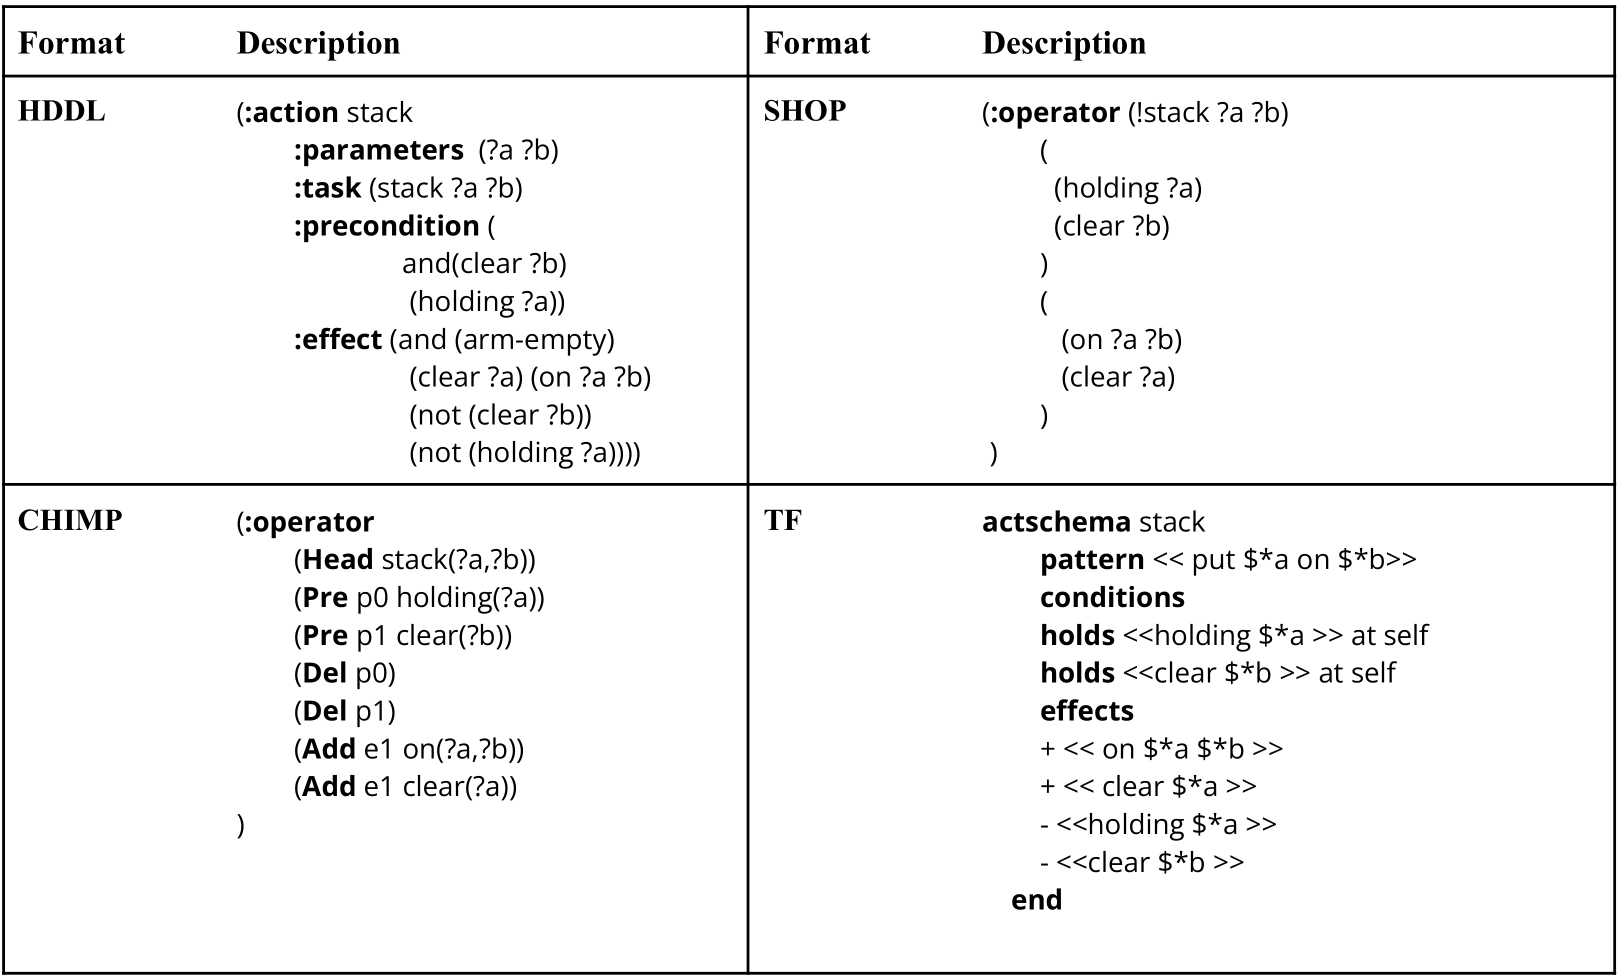
\includegraphics[width=\textwidth]{graphics/formats.png}
    \caption{The stack task from the block-world domain in different formats.}
    \label{fig:formats}
\end{figure}

There are also planners that use a programming language to describe the domain and problem rather than a specialized description language. This approach has the advantage that the planner can be directly integrated into the system using it without the need for a translation layer between the system and the planner. RAE\footnote{\url{https://github.com/patras91/rae_release}}, GTPyhop\footnote{\url{https://github.com/dananau/GTPyhop}} and FluidHTN\footnote{\url{https://github.com/ptrefall/fluid-hierarchical-task-network}} are all great examples of this approach.

\begin{Listing}
    \begin{lstlisting}[language=Python]
        def stack(s,b1,b2):
            if s.pos[b1] == 'hand' and s.clear[b2] == True:
                s.pos[b1] = b2
                s.clear[b1] = True
                s.holding['hand'] = False
                s.clear[b2] = False
                return s
    \end{lstlisting}
    \caption{The stack task from the block-world domain in GTPyhop.}
    \label{lst:StackPython}
\end{Listing}